\section{Background}
\label{sec:gpca-overview}

In this section, we provide a brief overview of an infusion pump system, its modeling and verification activities ~\cite{hilt2013, req2code} that is required to understand the formalization challenges described later in the paper. Infusion pumps are medical devices that are used to deliver controlled quantities of the drug into patient's body. Unfortunately, these devices have been involved in many incidents that triggered the need to strengthen their development practices~\cite{fda2010whitepaper}. In that context, our aim is to identify and demonstrate a rigours development approach of a generic infusion pump system using formal tools and techniques and release it publicly to be used as a reference for researchers, manufacturers and certification authorities.

\subsection {System Overview}
We considered a Generic Patient Controlled Analgesia Infusion Pump (GPCA), a special type of infusion pump that allows patients to self-administer a controlled amount of additional drug. %Figure~\ref{fig:gpca-overview} shows a GPCA device in a typical usage environment in which a clinician sets up the device and the patient receives the medication from the device through an intravenous needle according to the programmed prescription. To enhance safety of the device it is usually connected to a repository (hospital pharmacy database) that stores manufacturer provided drug limits.
% \begin{figure}[h!]
%    \centering
%    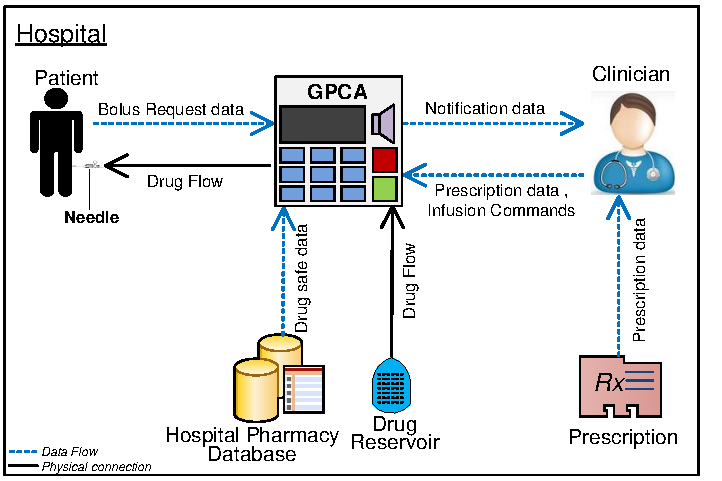
\includegraphics[scale=0.6]{images/Overview.pdf}
%    \caption{GPCA System Overview}
%    \label{fig:gpca-overview}
% \end{figure}
In order to analyse the problems associated with modern infusion pumps available in the market, created a model of similar complexity to current generation commercial infusion pumps. For instance, we considered three types of infusion options for drug delivery for the GPCA - (a) \emph{basal} infusion in which the drug is delivered at a constant (and usually low) rate for an extended period of
time, (b) \emph{intermittent bolus} infusion that delivers drug at a higher rate for a short duration at prescribed time intervals according to some therapy regimen, and (c) \emph{patient bolus} that delivers additional drug in response to a patient's request for more medication. In addition, we also included advanced safety features in the device to detect hazardous anomalies/behaviours and notifications for clinicians and mitigations via inhibiting infusion and/or other device operations.

\subsection {System Modeling and Verification}
\vspace{-0.07in}
Our interest with the GPCA is to develop and demonstrate a rigorous end-to-end development approach, using model based techniques. To begin with, we captured a reasonably complete set of overall system requirements using documentation patterns~\cite{mavin2009easy} and standard templates~\cite{IEEESRS} to simplify the task of formalizing requirements. During the modeling and verification the GPCA, to cope with its complexity, we followed a hierarchical decomposition approach that allows the modeling and verification to be systematically partitioned into smaller and more manageable tasks. In this approach, the system is hierarchically decomposed into a set of interconnected components (its architecture) and each component is allocated its own set of requirements. At the leaf level, in addition to the allocated requirements, the detailed behaviour of each component is modeled. This approach allows us to establish the requirements of the overall system by hierarchically verifying the component requirements at each level with respect to its model at that level.

We used a number of tools and techniques to implement this approach. We used the Architectural Analysis \& Design Language (AADL)~\cite{AADL:Overview} to capture the architecture of the GPCA (components and its interconnections) and an extension of the AADL language to capture formal requirements of the components (and system) until the leaf level. While the AADL notations allowed us to systematically allocate requirements to each component, it is not designed for constructing detailed behaviorial models. Hence, at the leaf level in addition to capturing its requirements, we separately modeled the behaviour of each component using MathWorks Simulink/Stateflow notation and tool~\cite{MathWorks} - a commonly used tool in the industry for behavioral modeling. To verify the hierarchical architecture driven requirements decomposition, we used a compositional reasoning tool named AGREE~\cite{NFM2012:CoGaMiWhLaLu}. Given the system architecture and the allocated requirements, AGREE hierarchically verifies if the system level guarantees holds as a logical consequence of its component requirements. To establish the leaf-level requirements, we used Simulink Design Verifier tool~\cite{MathWorks} and verified them with respect to their detailed behavioural model. Since we used two different tools, we recaptured the requirements from AGREE notation to a notation supported by Simulink Design Verifier, namely Embedded Matlab~\cite{MathWorks}. Fortunately, the rewriting was straightforward since both the notations have the same underlying semantics (that of synchronous dataflow languages). This approach and tool chain allowed us to rigorously demonstrate a scalable end-to-end system verification.

While our approach led to a complete verification of a hierarchically composed software architecture, the challenges in adopting the approach was not apparent until we applied it "at scale" over an extended period of time. In~\cite{hilt2013}, we demonstrated a proof of concept analysis on an early version of the model over a subset of system requirements (18 out of the 86 system requirements). In an effort to expand the application of our approach to the entire software of the GPCA, whose complexity and size was substantial, we formalized and verified all its requirements hierarchically. While there were 86 system requirements, we allocated 55 requirements to the software component and formalized them (rest of the system requirements were specific to the hardware). Since the software component was further decomposed into 8 components, we allocated 102 requirements altogether to its  components. In both the initial effort and the subsequent effort expanding the verification to the entire GPCA software, bringing on new team members, and validating our approach, we discovered a number of challenges that we elaborate in the next section.

%System 86
%SW - 55
%SW comp - 32+7+3+4+21+33 = 100

%To implement this approach to the entire GPCA (86 requirements) -- whose size and complexity is comparable to real industrial systems -- and assess its ease of use, we allocated the task of formalizing and verifying the requirements to a new team member, who although had experience using these tools, was not involved in developing the approach. We originally assumed this task was straightforward and planned 6 weeks for the activity. Unfortunately, we faced a number of challenges that considerably delayed the activity and lead to misplaced confidence about the system.
%
%
%when we started formalizing all the requirements of the infusion pump and verifying them we faced a number of challenges. The GPCA system has a total of 86 requirements and for the verification we selected 56 requirements that were relevant to the software of the GPCA. We allocated the task of formally formalizing and verifying these 56 requirements hierarchically in the GPCA model to one team member among us who was not involved in developing the approach.


%To model used
%
%
% that were manageable to model using Simulink/Stateflow tool and analyze using Simulink Design Verifier tool individually. We used Architectural Analysis \& Design Language (AADL) to capture the architecture of the GPCA (components and its interconnections).
%
%of the device and then modeled the behaviours of the system using
%
%To demonstrate such an development, it is absolutely crucial to have a suitable set of system requirements from which to start; to prove that the system (system model) does not pose a certain hazard, a precise description of the hazard avoidance or mitigation should be documented as requirements.
%
%we developed a requirements document for the GPCA by capturing requirements using various requirements discovery techniques.
%
% To demonstrate such an development,
%
%
%. We adopted an end-to-end model approach
%
%
% Since, the existing publicly available requirements documents did not meet our standards of completeness, consistency, and rigor, we began  developing a suitable requirements document for the GPCA. To discover the requirements of the GPCA, especially requirements related to continuous and continual aspects of the physical components used to build GPCA and its environment, we used a continuous domain model based approach. It helped us understand and precisely document the tolerances and allowances that had to be included in the system requirements, to account for inaccuracies of GPCA's physical components and environment. %While we documented the system level requirements using natural language, we had to move to a more formal notation as we begun the design and development of the system.
%
%To cope with complexity of modeling the GPCA, we hierarchically decomposed the system into various components. We used Architectural Analysis \& Design Language (AADL) to capture the architecture of the GPCA (components and its interconnections). The decomposition into components induces the need to identify how to precisely allocate requirements to each component in such a way that the system requirement is met. We captured GPCA and its component requirements using an extension of the AADL language that supports specification of formal textual requirements along with its respective components (and system) in the AADL model. This decomposition was not a simple requirements allocation task but an analysis activity in which we had to rigorously ascertain if the component requirements satisfies the system level requirements. For instance, we decomposed the GPCA's software (one of GPCA's components) into 8 sub-components to cope with complexity. To reason about the decomposition of GPCA software's requirements was not easy and hence we used a tool named AGREE~\cite{NFM2012:CoGaMiWhLaLu}. It is a compositional reasoning tool that helps automatically reason about the decomposition of requirements captured within AADL models.
%
%AGREE is based on assume-guarantee reasoning. In this style of reasoning, the requirements on components and system are captured as a \emph{Contracts}. A contract is an assume-guarantee pair in which ``guarantees" correspond to the promises that the component (or system) should satisfy, and ``assume'' correspond to the environmental constraints that are used (or necessary) to verify the promises. Given the system architecture and the contracts for both the system and its components, AGREE automatically verifies if the system level guarantees holds as a logical consequence of both component contracts and system level assumptions. While AGREE helped verify the correctness of GPCA software's contracts, it did so by assuming the correctness of the sub-component contracts. Hence, to verify if the sub-component contracts are indeed satisfied, we modeled and verified each of GPCA component using MathWorks tool suite.
%
%For modeling the GPCA software sub-components we used MathWorks Simulink/Stateflow and verified them using Simulink Design Verifier (SDV) tool. SDV verifies if requirements formalized as properties, using one of its supported notations, are satisfied by a Simulink model of the system. For the GPCA, we recaptured the component contracts in AGREE to properties using Embedded Matlab notation (supported by SDV) and verified if the component models satisfy them using SDV. We choose Embedded Matlab over the other options to formalize properties in SDV since its semantics to specify properties is the same as the the semantics of the notation used in AGREE to capture contracts. While our future plan is to automate the contract to property translation, due to time constraints we manually recaptured them for the GPCA.

%
%
%In addition, we also considered sophisticated validation features in the GPCA, such as  ensures if the entered values are within the safe limits as described in the hospital pharmacy database. In addition, the GPCA shall also have the capability to notify the clinician when exceptional conditions occur. These exceptional conditions include detecting anomalies in environment and unexpected device behaviours that may pose hazards to the patients. These exceptional conditions have varying levels of severity and expected system responses, such as buzzers, led lights and display of message and also inhibit infusion and other operations. In short, the GPCA system has three primary functions (1) deliver the drug based on the prescribed schedule and patient requests, (2) prevent hazards that may arise during its usage, and (3) monitor and notify the clinician of any exceptional conditions encountered. %The infusion, configuration and alarming capabilities are orthogonal to each other, that is, they function in parallel, but have the capability to affect each other's operation.
%
%Unfortunately, these devices have been involved in many incidents that have resulted in harm to the patient. Hence, The US Food and Drug Administration's (FDA)~\cite{fda2010whitepaper} in collaboration with the research community sought to pro-actively promote the development of infusion pumps that are safe to use. To contribute to this initiative, we developed an archetype of system development artifacts and demonstrated an end-to-end model based development approach for a generic
%infusion pump system, that could serve as a generic reference standard used by infusion pump manufactures and certification authorities.
%
